\section{Motorstyring }\label{sec:sec_motorstyring}
Målinger af vognens dynamik, der blev gennemgået i afsnit \ref{sec:sec_motoroverforelse}, er baseret på stepresponset af vognen ved en konstant spænding, men med faste strømbegrænsninger i intervaller.
Dette giver anledning til at vælge en motorstyring, der sørger for en konstant strøm til motoren.
Således vil udgangssignalet fra regulatoren i form af en reguleringsspænding, $V_{reg}$ omsættes i motorstyringen til den ønskede strøm $I_{reg}$, der igen giver den ønskede acceleration $a_v$ af vognen.  

\subsection{Design af motorregulering}
\begin{wrapfigure}{r}{0.5\textwidth}
	\centering
	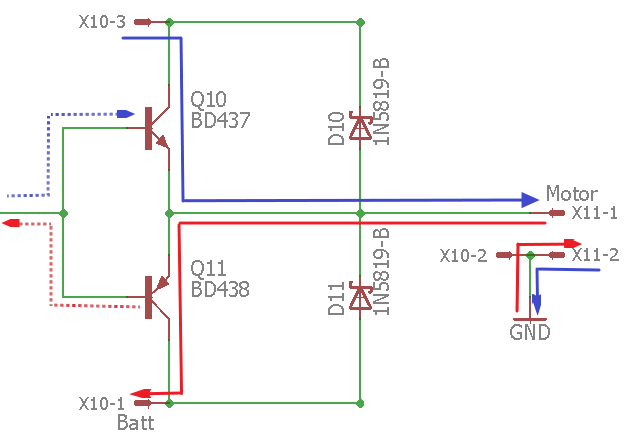
\includegraphics[width=.45\textwidth]{billeder/motor_bidirectional.png}
	\caption{Strømretninger ved positiv (blå) og negativ (rød) styresignal igennem BJT transistorne.}
	\label{fig:motor_bidirectional}
\end{wrapfigure}
Da DC-motoren er en kompleks enhed, hvis dynamik og opbygning ligger uden for omfanget af denne rapport. 
I figur \ref{fig:motor_diagram} ses det samlede kredsløb af motorreguleringen.
I motorstyringen anvendes en simpel feedback regulering af strømmen igennem en NPN \emph{(Q10)} og PNP \emph{(Q11)} transistor, således at forholdet mellem indgangssignalet og udgangsstrømmen til motoren holdes konstant.
Motorstyringen er opbygget som en såkaldt \textit{ Bi-directional DC motor driver} som gør det muligt at styre retningen af strømmen igennem motoren.
Således vil et positivt styresignal åbne for strømmen fra $+8V Batt$ igennem NPN transistoren \emph{(Q10)} ud til motoren, og et negativt styresignal vil åbne for strømmen fra $GND$ igennem PNP transistoren \emph{(Q11)} til $-8V Batt$, se figur \ref{fig:motor_bidirectional}.
\husk{JJ}{BJT valg, ref til datablad, og vigtige data som ligger til gunde for valg}

\begin{figure}[h!]
	\centering
	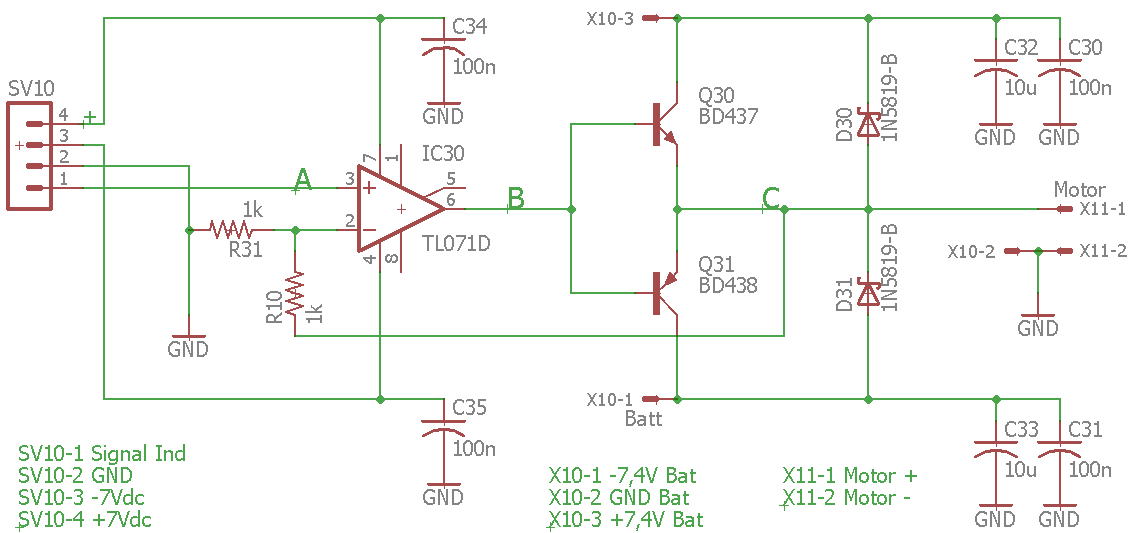
\includegraphics[width=1\textwidth]{billeder/motor_cont_schematic.png}
	\caption{Diagram af motor styringen}
	\label{fig:motor_diagram}
\end{figure}
\FloatBlock

For at håndtere de transiente spændingsudslag der måtte komme fra motor, idet den som spole er en induktiv belastning på udgangen.
Er der i kredsløbet anbragt to såkaldte \textit{flyback} eller friløbs dioder \emph{(D10)} og \emph{(D11)}.
Det er valgt at bruge en \textit{Schottky} \emph{1N5819}\cite{1N5819} diode, da denne har et lavere spændingsfald og en hurtigere \textit{reverse recovery}.

\subsection{Beregninger og dimensionering}
Da der i motorstyringen anvendes negativ feedback, kan dette bruges som udgangspunkt til at beregne forholdet mellem indgangssignalet til styringen og hvor stor strøm der kommer til at løbe igennem motoren.
Hvis der på indgang af motorstyringen, se figur \ref{fig:motor_diagram} punkt A, komme $+5 \si{\volt}$, vil op-amp'en (\emph{IC10}) gøre det den kan for at opnå at feedback signalet på dens negative indgang bliver lige så stort.
Det vil således betyde, at spændingen i punkt C vil være
\begin{align}
V_C = V_A \frac{R_{10}+R_{11}}{R_{11}} = 2V_A
\end{align}
Når motorens egenmodstand, der er målt til $R_{motor} = 3,2 \si{\ohm}$, kan strømmen igennem motoren kan således beregnes til maksimal
\begin{align}
I_{motor} =  \frac{2V_A}{R_{motor}} = \frac{10\si{\volt}}{3,2\si{\ohm}} = 3,125\si{\ampere} \label{eq:motor_VI}
\end{align}
Det er dog ikke muligt at opnå en spænding i punkt C på $V_C = 10\si{\volt}$, da forsyningen til motorstyringen kun er på $\pm 8 \si{\volt}$.
Der er også andre faktorer der begrænser spændingen i punkt C og derved giver en mindre strøm igennem motoren.
Forholdet i ligning \ref{eq:motor_VI}, vil dog an vendes til at beskrive motorstyringens dynamic
\begin{align}
H_{motor styring}(s) = \frac{V(s)}{I(s)} =\frac{R_{motor}}{2} = \frac{3,2}{2} = 1,6 \label{eq:motor_styr_trans}
\end{align}   

Under forsøg med den forover beskrevne motorstyring, viste det sig, at det ikke var muligt at få den strømstyrke ud til motoren som forventet.
Forsyningen til motorstyringen, blev derfor udskiftet med 2 stk. 9V batterier, således at \emph{(IC10)} blev forsynet med en højere spænding.
Med denne forbedring var det muligt at få en højere gate spænding på transistorne, og derved en højre $I_C$ strøm igennem dem.
 
\subsection{Overførelsesfunktion af motor}
For at bestemme dynamikken af DC-motoren opstilles en forenklet model af motoren.

\begin{figure}[h!]
	\centering
	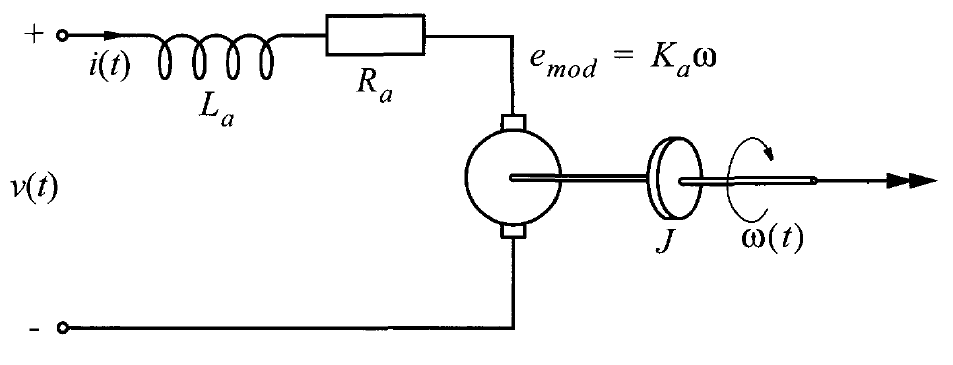
\includegraphics[width=.6\textwidth]{billeder/motor_model.png}
	\caption[Model af elektromotorisk system til brug ved modellering af motor]{Model af elektromotorisk system til brug ved modellering af motor\protect\footnotemark.}
	\label{fig:motor_model}
\end{figure}
\FloatBlock
\footnotetext{Figuren er tilrettet fra \cite[Figur 2.16, s. 52]{Reg2015}}

Ved at fastholde motoren, således at den mod-elektromotoriskekraft ($e_{mod}$) kan sættes til nul dvs. $\omega = 0$, er det muligt at måle motores induktans.
Modellen kan således omstilles som
\begin{align}
	v(t) = R_ai(t) + L_a\dfrac{di(t)}{dt}
\end{align}
Måling af strømmen igennem motoren er forstaget over en $0,2 \si{\ohm}$ test-modstand
\footnote{Modstand med meget lille induktans}.
Motorens egen modstand er målt til $R_{motor} = 3,2 \si{\ohm}$, hvilket giver en samlet modstand på $R_a = R_{test} + R_{motor} = 3,4 \si{\ohm}$ i test opstillingen. 
\begin{figure}[h!]
	\centering
	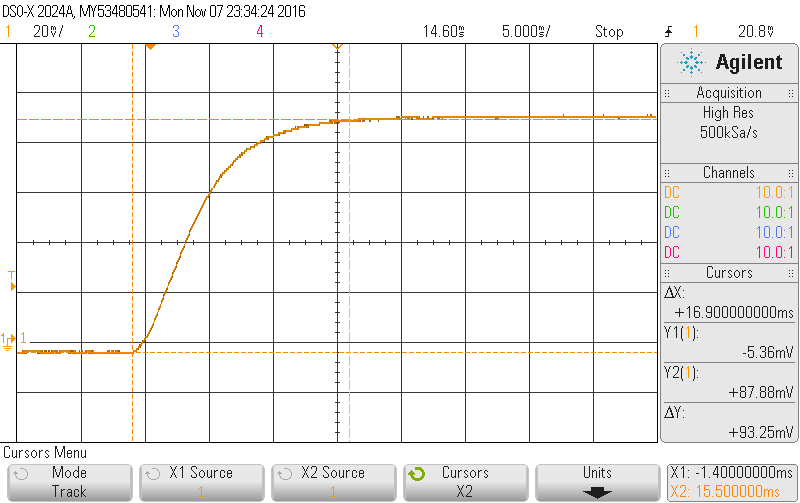
\includegraphics[width=.8\textwidth]{billeder/motor_L.png}
	\caption{Måling af transient forløb for strømmen igennem DC-motor.}
	\label{fig:motor_dynamik_scoop}
\end{figure}
Tidskonstanten for ladning af en spole er, $\tau = \frac{L}{R}$.
For at bestemme $L$, måles tiden $t$ ved $5\tau$ som er ved
\begin{align}
	\% opladning = \left( 1 - \frac{1}{e^{t/\tau}} \right) \cdot 100\% \Rightarrow  \left( 1 - \frac{1}{e^{t/5}} \right) \cdot 100 \approx 99,32\% 
\end{align}
derefter kan $L_a$ bestemmes som, ved aflæst tid på $16,9\si{\milli\second}$ i fig. \ref{fig:motor_dynamik_scoop} 
\begin{align}
	5\tau = \frac{L_a}{R_a} \Rightarrow L_a = 16,9\si{\milli\second} \cdot 3,4 \si{\ohm} = 57,5 \si{\milli\henry}
\end{align}
Overførelsesfunktion for motoren opstilles som, hvori ligning \ref{eq:motor_styr_trans} for $H_{motorstyring}$ medtages
\begin{align}
H_{motor} &= \frac{V_o}{V_i} \cdot H_{motorstyring} = \frac{s L_a}{s L_a + R_{motor}} \cdot H_{motorstyring} = \frac{ \frac{L_a}{R_{motor}}s}{ \frac{L_a}{R_{motor}}s +1} \cdot H_{motorstyring} \\
 &= 1,6 \cdot \frac{\num{18E-3}s}{\num{18E-3}s +1}  \label{eq:motor_trans}
\end{align}  



